\section{Intersecting Families}

Sperner's theorem came out of forbidding one hyper-edge to sit inside another. Forbidding the opposite---a pair of hyper-edges that miss each other entirely---turns out to have a much more interesting answer, and it is the one we spend this section on.

\begin{boxdefinition}[Intersecting]
    We say that a $k$-uniform hypergraph $H$ is \textbf{intersecting} if $\forall h_1, h_2 \in \H$, $h_1 \cap h_2 \ne \emptyset$.
\end{boxdefinition}

The question is: how big can an intersecting $k$-uniform hypergraph on $n$ vertices be? Ie, how many hyper-edges can it have? Small $k$ is worth doing by hand, and as long as $n \geq 2k$ every case points the same way---until the last one, where dropping that assumption is exactly the point.

\begin{itemize}
    \item $k = 1$: we can see that the maximum number of edges must be $1$.
    \item $k = 2$: the maximum number of edges is $n - 1$, achieved by the `star graph'
    \begin{center}
        \begin{tikzpicture}
            \stargraph[1.15]{7}
        \end{tikzpicture}
    \end{center}
    \item $k = 3$: $\binom{n-1}{2}$, achieved by fixing one vertex that lies in everything and choosing $2$ more.
    \item $k \leq \frac{n}{2}$: $\binom{n-1}{k-1}$ by exactly the same strategy.
    \item $k > \frac{n}{2}$: we can do better! $\binom{n}{k}$ works because of something involving pigeons and holes.
\end{itemize}

The middle of that list is the general answer, and the bottom of it is why $n \geq 2k$ has to be assumed to get one.

\begin{boxtheorem}[\Erdos-Ko-Rado] \label{Ch1:Thm:EKR}
    If $n \geq 2k$, and $H$ is an intersecting $k$-uniform hypergraph on $n$ vertices, then the number of hyper-edges of $H$ is $\leq \binom{n-1}{k-1}$. Moreover, if $n \geq 2k + 1$, then the (``unique'') extremal example is given by all $k$-subsets containing a fixed vertex.
\end{boxtheorem}

% [CORRECTED] was: "some partition of $H$ into subsets of size $k$", and "$h \in \pi(f)$" in the display --- what the
% argument needs is a partition of the vertex set rather than of the edge set: the $n / k$ in the expectation below counts
% its blocks, and $X \leq 1$ holds because they are pairwise disjoint. And $h$ and $\pi(f)$ are both $k$-sets of vertices,
% so the relation between them is $=$, not $\in$; the display two lines down already writes $\Pr\of{h = \pi(f)}$.
As a warmup case, let's assume that $k \mid n$. Suppose $H$ is intersecting. Let $\calF$ denote some partition of $[n]$ into $n / k$ subsets of size $k$ (so $\calF$ is fundamentally a collection of subsets).
\begin{align*}
    X = \abs{\setst{h \in \H}{h = \pi(f) \text{ for some } f \in \calF}}
\end{align*}
where $\pi \in S_n$ is a permutation chosen uniformly at random.

Note that $X \leq 1$. Let's now compute its expected value.
\begin{align*}
    \E\of{X} &= \sum_{h \in \H} \sum_{f \in \calF} \Pr\of{h = \pi(f)} \\
    &= \abs{\H} \cdot \frac{n}{k} \cdot \frac{1}{\binom{n}{k}}
\end{align*}
So since $X \leq 1$, we conclude that
\begin{align*}
    \abs{\H} \cdot \frac{n}{k} \cdot \frac{1}{\binom{n}{k}} \leq \E\of{X} \leq 1
\end{align*}
Rearranging gives us that
\begin{align*}
    \abs{\H} \leq \binom{n}{k} \cdot \frac{k}{n} = \binom{n-1}{k-1}
\end{align*}

Now let's prove the result in full generality. The random permutation survives, but the partition into $n / k$ blocks does not, and what replaces it is a cycle.

\begin{boxlnotation}
    Lay the $n$ vertices out around a circle. A \textbf{$k$-interval} of that cycle is a set of $k$ vertices occupying consecutive positions on it, and $\calF_{\pi}$ will denote the collection of all of them when the vertices are laid out in the order $\pi(1), \pi(2), \ldots, \pi(n)$.
\end{boxlnotation}

\begin{figure}[H]
    \centering
    \begin{tikzpicture}
        \cyclearc[1.5]{11}{4}{10}
    \end{tikzpicture}
\end{figure}

There are $n$ intervals in $\calF_{\pi}$, one starting at each vertex, and---this is the whole point of moving to a cycle---very few of them can pairwise intersect.

% [CORRECTED] was: "The maximum number of intersecting edges in $F$ is $k$. Moreover, any collection $C$ of $k$
% intersecting edges in $F$, $C$ must be the collection of all edges that include some fixed vertex." --- the second
% half needs $n \geq 2k + 1$, which that sentence does not carry. At $n = 2k$ it fails for every $k \geq 3$; the
% counterexample recorded after the proof is the smallest one.
\begin{boxlemma} \label{Ch1:Lemma:Intersecting_Intervals}
    Let $n \geq 2k$. Any collection $\calC \subseteq \calF_{\pi}$ of pairwise intersecting $k$-intervals has $\abs{\calC} \leq k$. Moreover, if $n \geq 2k + 1$ and $\abs{\calC} = k$, then $\calC$ is the collection of all the $k$-intervals containing some one vertex.
\end{boxlemma}
% [FILLED] the lecture asserted both halves of this without proof; the proof below was supplied
\begin{proof}
    Assume $\calC$ is nonempty and fix some $I \in \calC$, occupying positions $a, a + 1, \ldots, a + k - 1$. For $i = 1, \ldots, k - 1$, let $A_i$ be the interval ending at position $a + i - 1$ and let $B_i$ be the one starting at position $a + i$. Every interval other than $I$ that meets $I$ is one of these $2k - 2$: an interval meets $I$ exactly when it starts at one of the $2k - 1$ positions $a - k + 1, \ldots, a + k - 1$, and the $A_i$ take the $k - 1$ of those before $a$ while the $B_i$ take the $k - 1$ after it. Now $A_i$ and $B_i$ between them occupy the $2k$ consecutive positions $a + i - k, \ldots, a + i + k - 1$, which are distinct because $n \geq 2k$, so $A_i \cap B_i = \emptyset$ and $\calC$ can contain at most one of the two. Taking $I$ together with one interval from each of the $k - 1$ pairs gives $\abs{\calC} \leq k$.

    Suppose now that $n \geq 2k + 1$ and $\abs{\calC} = k$, so that $\calC$ holds exactly one of $A_i, B_i$ for every $i$. It cannot hold both $A_i$ and $B_{i+1}$: those occupy positions $a + i - k, \ldots, a + i - 1$ and $a + i + 1, \ldots, a + i + k$, which lie among $2k + 1$ consecutive positions and so are distinct, leaving the two intervals disjoint. So as soon as some $B_j$ lies in $\calC$ so does every $B_i$ with $i < j$, and hence there is an $m$ with
    \begin{align*}
        \calC = \set{A_{k-1}, \ldots, A_{m+1}, I, B_1, \ldots, B_m}
    \end{align*}
    Reading off where each of those starts, they are the intervals starting at positions $a + m + 1 - k, \ldots, a + m$, which is a run of $k$ consecutive positions---and the intervals starting there are precisely the ones containing the vertex at position $a + m$.
\end{proof}

The hypothesis $n \geq 2k + 1$ does real work in that second half: on $C_6$ the three $3$-intervals $\set{1, 2, 3}$, $\set{3, 4, 5}$ and $\set{5, 6, 1}$ pairwise intersect, and there are $k = 3$ of them, but no vertex lies in all three.

\begin{proof}[Proof of the bound in \Cref{Ch1:Thm:EKR}]
    Choose $\pi \in S_n$ uniformly at random and set
    \begin{align*}
        X = \abs{\setst{h \in \H}{h \in \calF_{\pi}}}
    \end{align*}
    The intervals being counted here are hyper-edges of $H$, so they pairwise intersect, and by \Cref{Ch1:Lemma:Intersecting_Intervals} it is always true that $X \leq k$. Now, let's compute the expectation of $X$.
    % [FILLED] the lecture broke off at ``let's compute the expectation of $X$''; the computation and the conclusion below were supplied
    \begin{align*}
        \E\of{X} = \sum_{h \in \H} \Pr\of{h \in \calF_{\pi}}
    \end{align*}
    A given $h$ is an interval of the randomly ordered cycle exactly when $\pi$ lays its $k$ elements out consecutively, and we can count the $\pi$ that do so. There are $n$ places for the interval to start, $k!$ ways of arranging $h$ within it and $\parenth{n - k}!$ ways of arranging the other $n - k$ vertices, and no $\pi$ gets counted twice, since an interval determines where it starts. So
    \begin{align*}
        \Pr\of{h \in \calF_{\pi}} = \frac{n \cdot k! \parenth{n - k}!}{n!} = \frac{n}{\binom{n}{k}}
    \end{align*}
    and hence
    \begin{align*}
        \abs{\H} \cdot \frac{n}{\binom{n}{k}} = \E\of{X} \leq k
    \end{align*}
    Rearranging,
    \begin{align*}
        \abs{\H} \leq \frac{k}{n} \binom{n}{k} = \binom{n-1}{k-1}
    \end{align*}
\end{proof}

That argument has slack in exactly one place, and at $\abs{\H} = \binom{n-1}{k-1}$ there is none left: $X$ is then equal to $k$ for every ordering rather than merely on average. Once $n \geq 2k + 1$, so that the second half of \Cref{Ch1:Lemma:Intersecting_Intervals} is available, every ordering of the cycle hands us a run of $k$ intervals all of which are hyper-edges---and that pins $\H$ down completely. The following is the ``moreover'' of \Cref{Ch1:Thm:EKR}, made precise.

% [CORRECTED] was: "If $\abs{\H} = \binom{n-1}{k-1}$ and $n \geq 2k + 1$, then the extremal example ...", with no
% hypothesis on $H$ at all. Read as the free-standing statement a boxed theorem is, that is false: it would make any
% $\binom{n-1}{k-1}$ subsets of $[n]$ a star. Both hypotheses are load-bearing --- without $k$-uniformity the
% cardinality is no longer the star's, and without intersecting nothing forces a common vertex.
\begin{boxtheorem} \label{Ch1:Thm:EKR_Extremal}
    Let $H$ be an intersecting $k$-uniform hypergraph on $n$ vertices. If $\abs{\H} = \binom{n-1}{k-1}$ and $n \geq 2k + 1$, then the extremal example is the obvious one: there is a vertex $x$ such that $\H$ consists of precisely the $k$-subsets of $[n]$ that contain $x$.
\end{boxtheorem}

\begin{figure}[H]
    \centering
    \begin{tikzpicture}
        \cyclefan[1.5]{11}{4}{1}
        \node[anchor = north] at (90:1.34) {$x$};
    \end{tikzpicture}
\end{figure}

Whatever order we lay the vertices out in, the picture looks like the one above: the hyper-edges we can see on the cycle are the $k$ intervals through one distinguished vertex, drawn here as concentric arcs. All the work is in showing that the distinguished vertex does not move when the order changes.

% [FILLED] the statement broke off mid-sentence and the lecture sketched the proof in a line; the completion above and the argument below were supplied

Here is the picture to keep in mind. Swapping two neighbors on the cycle disturbs only two of its $n$ intervals---the one ending at the first of them and the one starting at the second, each of which holds exactly one of the pair---and every other interval keeps its vertices. So at least $k - 1$ of the $k$ arcs through $x$ are still hyper-edges and still intervals after the swap, and $k - 1$ consecutive arcs leave the new fan almost no room to sit anywhere else. The proof below is the bookkeeping that turns ``almost'' into ``none''.

\begin{figure}[H]
    \centering
    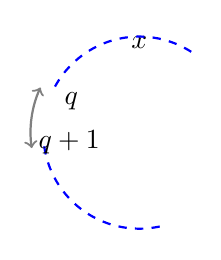
\begin{tikzpicture}
        \cyclefan[1.5]{11}{4}{1}
        \node[anchor = north] at (90:1.34) {$x$};
        \draw[thick, dashed, blue] ({90 - 360 / 11}:1.22) arc ({90 - 360 / 11}:{90 + 360 * 2 / 11}:1.22);
        \draw[thick, dashed, blue] ({90 + 360 * 3 / 11}:1.22) arc ({90 + 360 * 3 / 11}:{90 + 360 * 6 / 11}:1.22);
        \draw[<->, thick, gray] ({90 + 360 * 2 / 11}:1.38) arc ({90 + 360 * 2 / 11}:{90 + 360 * 3 / 11}:1.38);
        \node at ({90 + 360 * 2 / 11}:0.95) {$q$};
        \node at ({90 + 360 * 3 / 11}:0.9) {$q + 1$};
    \end{tikzpicture}
\end{figure}

Here $n = 11$ and $k = 4$. The two dashed intervals are the ones the swap of positions $q$ and $q + 1$ disturbs; one of them is among the four hyper-edges through $x$ and the other is not, and the remaining three arcs are untouched.

\begin{proof}[Proof of \Cref{Ch1:Thm:EKR_Extremal}]
    Run the argument above again, this time at equality. If $\abs{\H} = \binom{n-1}{k-1}$, then
    \begin{align*}
        \E\of{X} = \binom{n-1}{k-1} \cdot \frac{n}{\binom{n}{k}} = k
    \end{align*}
    and we already know that $X \leq k$ whatever $\pi$ is. There are finitely many $\pi$ and each is equally likely, so a mean of $k$ under a ceiling of $k$ leaves nothing to spare: $X = k$ for every single $\pi$. However we lay the $n$ vertices out around a cycle, then, exactly $k$ of that cycle's $k$-intervals are hyper-edges of $H$, and by \Cref{Ch1:Lemma:Intersecting_Intervals} those $k$ intervals are the intervals through a single vertex---one vertex and no more, since the outermost two of them share only it. Write $x_{\pi}$ for that vertex. For $k = 1$ an intersecting family is a single hyper-edge and the theorem is immediate, so assume from here that $k \geq 2$.

    It remains to see that $x_{\pi}$ does not depend on $\pi$, and one adjacent transposition at a time is enough. Fix an ordering, put $x = x_{\pi}$ at position $0$ and number the other positions $1, \ldots, n - 1$ round the circle, and let $I_j$ be the interval occupying \emph{positions} $j, j + 1, \ldots, j + k - 1$, indices read modulo $n$. The intervals through position $c$ are $I_{c-k+1}, \ldots, I_{c}$, so the hyper-edges of this ordering are exactly $I_{-(k-1)}, \ldots, I_{0}$. Transposing the vertices at adjacent positions $q$ and $q + 1$, neither of them position $0$, changes which vertices occupy $I_j$ exactly when $I_j$ holds one of those two positions and not the other---which happens for $j = q + 1$ and for $j = q - k + 1$, and for no other $j$.

    So the new ordering's hyper-edges, again the intervals through a single position $c$, agree with $I_{-(k-1)}, \ldots, I_{0}$ outside those two indices. But two runs of $k$ consecutive indices whose right-hand ends sit $c$ apart differ in $2\min\of{\abs{c}, k}$ places, where $\abs{c}$ is the distance from $c$ to $0$ measured around the circle, so $c \neq 0$ would force $\abs{c} = 1$, and the two indices they differ in are then $\set{-(k-1), 1}$ if $c = 1$ and $\set{-k, 0}$ if $c = -1$. Either set would have to be $\set{q - k + 1, q + 1}$. Both pairs differ by $k$, and matching them in the only order that does not ask for $-k \equiv k \pmod{n}$ (which is impossible, as $n > 2k$) gives $q = 0$ in the first case and $q = -1$ in the second. Both are excluded, so $c = 0$: the distinguished vertex is the one at position $0$, which the transposition left where it was.

    Adjacent transpositions avoiding position $0$ generate every arrangement of the other $n - 1$ vertices around the circle, and each one leaves the distinguished vertex at position $0$ for the next to start from, so the paragraph above applies afresh along the whole chain. Rotating or reflecting a layout leaves its intervals, and hence $x_{\pi}$, alone---so every $\pi$ can first be turned until $x$ sits at position $0$, and $x_{\pi} = x$ for all of them. Take any $k$-subset $h$ of $[n]$ containing $x$, and lay the vertices out with the elements of $h$ consecutive: then $h$ is an interval containing $x$, so $h \in \H$. There are $\binom{n-1}{k-1}$ such $h$, which is exactly $\abs{\H}$, so they are all of it.
\end{proof}